
\documentclass[spanish, 11pt]{exam}

%These tell TeX which packages to use.
\usepackage{array,epsfig}
\usepackage{amsmath, textcomp}
\usepackage{amsfonts}
\usepackage{amssymb}
\usepackage{amsxtra}
\usepackage{amsthm}
\usepackage{mathrsfs}
\usepackage{color}
\usepackage{multicol, xparse}
\usepackage{verbatim}


\usepackage[utf8]{inputenc}
\usepackage[spanish]{babel}
\usepackage{eurosym}

\usepackage{graphicx}
\graphicspath{{../img/}}



\printanswers
\nopointsinmargin
\pointformat{}

%Pagination stuff.
%\setlength{\topmargin}{-.3 in}
%\setlength{\oddsidemargin}{0in}
%\setlength{\evensidemargin}{0in}
%\setlength{\textheight}{9.in}
%\setlength{\textwidth}{6.5in}
%\pagestyle{empty}

\let\multicolmulticols\multicols
\let\endmulticolmulticols\endmulticols
\RenewDocumentEnvironment{multicols}{mO{}}
 {%
  \ifnum#1=1
    #2%
  \else % More than 1 column
    \multicolmulticols{#1}[#2]
  \fi
 }
 {%
  \ifnum#1=1
  \else % More than 1 column
    \endmulticolmulticols
  \fi
 }
\renewcommand{\solutiontitle}{\noindent\textbf{Sol:}\enspace}

\newcommand{\samedir}{\mathbin{\!/\mkern-5mu/\!}}

\newcommand{\class}{4º ESO}
\newcommand{\examdate}{\today}

\newcommand{\tipo}{A}


\newcommand{\timelimit}{50 minutos}



\pagestyle{head}
\firstpageheader{
\includegraphics[width=0.2\columnwidth]{header_left}}{\textbf{Departamento de Matemáticas\linebreak \class}\linebreak \examnum}{
\includegraphics[width=0.1\columnwidth]{header_right}}
\runningheader{\class}{\examnum}{Página \thepage\ of \numpages}
\runningheadrule

\newcommand{\examnum}{Autoevaluación - Trimestre 3}
\begin{document}
\begin{questions}

%\question Representa y calcula las coordenadas de las siguientes combinaciones de $\overrightarrow{u}$ y $\overrightarrow{v}$:\begin{parts} \part[1] $2 \overrightarrow{u} - 3 \overrightarrow{v}$, $- 2 \overrightarrow{u}$, $- 2 \overrightarrow{u} - 2 \overrightarrow{v}$. Siendo $\overrightarrow{u}$ y $\overrightarrow{v}$: \\ \scalebox{.65}{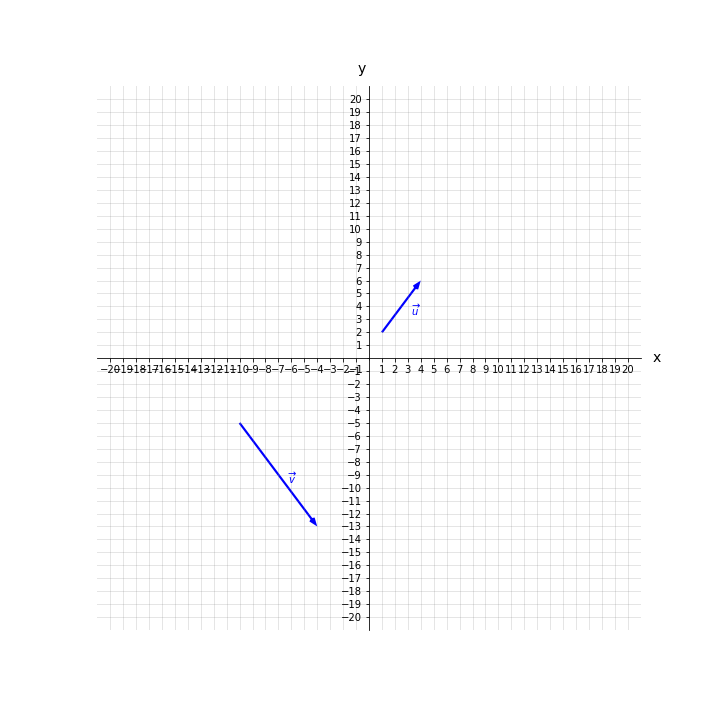
\includegraphics[width=1\columnwidth]{comb_vectores_0.png}}\begin{solution} $2 \overrightarrow{u} - 3 \overrightarrow{v}$, $- 2 \overrightarrow{u}$, $- 2 \overrightarrow{u} - 2 \overrightarrow{v}$\end{solution} \end{parts}


\question Las calificaciones de un grupo de 34 alumnos han sido: 9 6 5 0 1 5 7 9 10 7 5 1 2 5 7 6 3 4 6 8 8 6 4 4 6 5 3 5 7 7 8 7 2 2. Realiza una tabla de frecuencias. Realiza un diagrama de barras y un polígono de frecuencias. Calcular los parámetros de centralización. Calcular los parámetros de posición P70, Q1, Q3, D4. Calcular los parámetros de dispersión
\begin{solution}
$\begin{tabular}{rrrrrrr}
\hline
   x\_i &   f\_i &   F\_i &       h\_i &       H\_i &      \%\_i &      \%A\_i \\
\hline
     0 &     1 &     1 & 0.0294118 & 0.0294118 &  2.94118 &   2.94118 \\
     1 &     2 &     3 & 0.0588235 & 0.0882353 &  5.88235 &   8.82353 \\
     2 &     3 &     6 & 0.0882353 & 0.176471  &  8.82353 &  17.6471  \\
     3 &     2 &     8 & 0.0588235 & 0.235294  &  5.88235 &  23.5294  \\
     4 &     3 &    11 & 0.0882353 & 0.323529  &  8.82353 &  32.3529  \\
     5 &     6 &    17 & 0.176471  & 0.5       & 17.6471  &  50       \\
     6 &     5 &    22 & 0.147059  & 0.647059  & 14.7059  &  64.7059  \\
     7 &     6 &    28 & 0.176471  & 0.823529  & 17.6471  &  82.3529  \\
     8 &     3 &    31 & 0.0882353 & 0.911765  &  8.82353 &  91.1765  \\
     9 &     2 &    33 & 0.0588235 & 0.970588  &  5.88235 &  97.0588  \\
    10 &     1 &    34 & 0.0294118 & 1         &  2.94118 & 100       \\
\hline
\end{tabular}$\\ 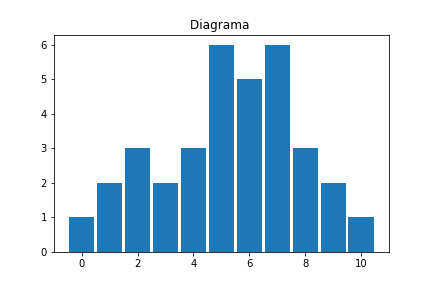
\includegraphics[width=1\columnwidth]{diagrama0} \\ $\left\{ Me : 5.5, \  Mo : \left( [5], \  [6]\right), \  media : 5.29\right\}$ \\$\left\{ D4 : 5.0, \  P70 : 7.0, \  Q1 : 4.0, \  Q3 : 7.0\right\}$ \\$\left\{ C.V : 0.46, \  desv.tip : 2.46, \  rango : 10, \  var : 6.03\right\}$
\end{solution}


\question Calcula el punto medio del segmento que une los puntos:
\begin{multicols}{3}
\begin{parts} \part[1] $A\left( -5, \  1\right) y \ B\left( 3, \  7\right)$ \begin{solution} $M\left( -1, \  4\right)$\end{solution} \part[1] $A\left( 4, \  -1\right) y \ B\left( -2, \  -4\right)$ \begin{solution} $M\left( 1, \  - \frac{5}{2}\right)$\end{solution} \part[1] $A\left( 1, \  -5\right) y \ B\left( 5, \  -3\right)$ \begin{solution} $M\left( 3, \  -4\right)$\end{solution} \end{parts} 
\end{multicols}

\question Halla el valor de z para que los puntos A  , B    y C estén alineados. Siendo:
\begin{multicols}{3}
\begin{parts} \part[1] $A\left( 1, \  -2\right)$, $B \left( 3, \  1\right)$ y $C\left( 4, \  z\right)$ \begin{solution} $Point2D\left(2, 3\right)\parallel Point2D\left(3, z + 2\right) \to z=\left[ \frac{5}{2}\right]$\end{solution} \part[1] $A\left( 2, \  -4\right)$, $B \left( 5, \  3\right)$ y $C\left( 6, \  z\right)$ \begin{solution} $Point2D\left(3, 7\right)\parallel Point2D\left(4, z + 4\right) \to z=\left[ \frac{16}{3}\right]$\end{solution} \part[1] $A\left( 5, \  4\right)$, $B \left( -5, \  -2\right)$ y $C\left( 1, \  z\right)$ \begin{solution} $Point2D\left(-10, -6\right)\parallel Point2D\left(-4, z - 4\right) \to z=\left[ \frac{8}{5}\right]$\end{solution} \end{parts} 
\end{multicols}


\question Calcula el punto simétrico:
\begin{multicols}{2}
\begin{parts} \part[1] De $A\left( 7, \  6\right)$ respecto  de  $M\left( 2, \  1\right)$ \begin{solution} $Point2D\left(\dfrac{x}{2} + \dfrac{7}{2}, \dfrac{y}{2} + 3\right) = Point2D\left(2, 1\right)\to A'\left(-3,-4\right)$\end{solution} \part[1] De $A\left( 5, \  -3\right)$ respecto  de  $M\left( 1, \  3\right)$ \begin{solution} $Point2D\left(\dfrac{x}{2} + \dfrac{5}{2}, \dfrac{y}{2} - \dfrac{3}{2}\right) = Point2D\left(1, 3\right)\to A'\left(-3,9\right)$\end{solution} \part[1] De $A\left( 6, \  -5\right)$ respecto  de  $M\left( -3, \  2\right)$ \begin{solution} $Point2D\left(\dfrac{x}{2} + 3, \dfrac{y}{2} - \dfrac{5}{2}\right) = Point2D\left(-3, 2\right)\to A'\left(-12,9\right)$\end{solution} \part[1] De $A\left( -6, \  -2\right)$ respecto  de  $M\left( 4, \  1\right)$ \begin{solution} $Point2D\left(\dfrac{x}{2} - 3, \dfrac{y}{2} - 1\right) = Point2D\left(4, 1\right)\to A'\left(14,4\right)$\end{solution} \end{parts}
\end{multicols}

\question Halla las coordenadas del punto D, de modo que ABCD sea un paralelogramo siendo\begin{parts} \part[1] Siendo $A$, $B$ y $C$ respectivamente: $\left( 2, \  -3\right) $, $\left( 0, \  1\right) $, $\left( 4, \  3\right)$\begin{solution} $\overrightarrow{AB} = \overrightarrow{DC} \to Point2D\left(-2, 4\right) = Point2D\left(4 - x, 3 - y\right) \to D\left( 6, \  -1\right)$\end{solution} \part[1] Siendo $A$, $B$ y $C$ respectivamente: $\left( 1, \  -1\right) $, $\left( 1, \  1\right) $, $\left( 2, \  3\right)$\begin{solution} $\overrightarrow{AB} = \overrightarrow{DC} \to Point2D\left(0, 2\right) = Point2D\left(2 - x, 3 - y\right) \to D\left( 2, \  1\right)$\end{solution} 
%\part[1] Siendo $A$, $B$ y $C$ respectivamente: $\left( -2, \  -3\right) $, $\left( -2, \  2\right) $, $\left( 5, \  4\right)$\begin{solution} $\overrightarrow{AB} = \overrightarrow{DC} \to Point2D\left(0, 5\right) = Point2D\left(5 - x, 4 - y\right) \to D\left( 5, \  -1\right)$\end{solution} 
\end{parts} 

\question Escribe las ecuaciones vectorial, paramétricas, en forma continua y explícita de la recta que:\begin{parts} \part[1] Pasa por el punto $P$ y tiene por vector dirección $\overrightarrow{d}$ respectivamente: $\left( 3, \  -1\right) $, $\left( -2, \  5\right)$\begin{solution} Solución orientativa: $Point2D\left(x, y\right) = Point2D\left(3 - 2 t, 5 t - 1\right) \to - 5 x - 2 y + 13 = 0 \to y = \dfrac{13}{2} - \dfrac{5 x}{2}$\end{solution} \part[1] Pasa por el punto $P$ y tiene por vector dirección $\overrightarrow{d}$ respectivamente: $\left( 1, \  -3\right) $, $\left( 3, \  -2\right)$\begin{solution} Solución orientativa: $Point2D\left(x, y\right) = Point2D\left(3 t + 1, - 2 t - 3\right) \to 2 x + 3 y + 7 = 0 \to y = - \dfrac{2 x}{3} - \dfrac{7}{3}$\end{solution} \part[1] Pasa por el punto $P$ y tiene por vector dirección $\overrightarrow{d}$ respectivamente: $\left( 2, \  3\right) $, $\left( -3, \  5\right)$\begin{solution} Solución orientativa: $Point2D\left(x, y\right) = Point2D\left(2 - 3 t, 5 t + 3\right) \to - 5 x - 3 y + 19 = 0 \to y = \dfrac{19}{3} - \dfrac{5 x}{3}$\end{solution} \end{parts}

\question Escribe las ecuaciones vectorial, paramétricas, en forma continua y explícita de la recta que:\begin{parts} \part[1] Pasa por los puntos $P$ y $Q$ respectivamente: $\left( 2, \  -1\right) $, $\left( -2, \  5\right)$\begin{solution} Solución orientativa: $Point2D\left(x, y\right) = Point2D\left(2 - 4 t, 6 t - 1\right) \to - 6 x - 4 y + 8 = 0 \to y = 2 - \dfrac{3 x}{2}$\end{solution} \part[1] Pasa por los puntos $P$ y $Q$ respectivamente: $\left( 2, \  -3\right) $, $\left( 3, \  -2\right)$\begin{solution} Solución orientativa: $Point2D\left(x, y\right) = Point2D\left(t + 2, t - 3\right) \to - x + y + 5 = 0 \to y = x - 5$\end{solution} 
%\part[1] Pasa por los puntos $P$ y $Q$ respectivamente: $\left( -4, \  3\right) $, $\left( -3, \  5\right)$\begin{solution} Solución orientativa: $Point2D\left(x, y\right) = Point2D\left(t - 4, 2 t + 3\right) \to - 2 x + y - 11 = 0 \to y = 2 x + 11$\end{solution} 
\end{parts} 

\question Calcula la recta $s$ que:
%\begin{multicols}{2}
\begin{parts} \part[1] pasa por P$\left( 3, \  1\right)$ y es paralela a $r \equiv 4 x - 2 y + 1 = 0$\begin{solution} $s\equiv y = 2 x - 5$\end{solution} \part[1] pasa por P$\left( -1, \  2\right)$ y es paralela a $r \equiv 2 x - 3 y + 1 = 0$\begin{solution} $s\equiv y = \dfrac{2 x}{3} + \dfrac{8}{3}$\end{solution} \end{parts} 
%\end{multicols}

\question Calcula la recta $s$ que:\begin{parts} \part[1] pasa por P$\left( -1, \  2\right)$ y es perpendicular a $\overrightarrow{v}\left( -2, \  1\right)$\begin{solution} $s\equiv 2 x - y + 4 = 0$\end{solution} \part[1] pasa por P$\left( 1, \  -2\right)$ y es perpendicular a $\overrightarrow{v}\left( 5, \  -4\right)$\begin{solution} $s\equiv - 5 x + 4 y + 13 = 0$\end{solution} \part[1] pasa por P$\left( 1, \  -2\right)$ y es perpendicular a $\overrightarrow{v}\left( -1, \  0\right)$\begin{solution} $s\equiv x - 1 = 0$\end{solution} \end{parts}

\question Calcula la recta $s$ que:
\begin{multicols}{2}
\begin{parts} \part[1] pasa por P$\left( 3, \  1\right)$ y es perpendicular a $r \equiv 4 x - 2 y + 1 = 0$\begin{solution} $s\equiv y = \dfrac{5}{2} - \dfrac{x}{2}$\end{solution} \part[1] pasa por P$\left( -1, \  2\right)$ y es perpendicular a $r \equiv 2 x - 3 y + 1 = 0$\begin{solution} $s\equiv y = \dfrac{1}{2} - \dfrac{3 x}{2}$\end{solution} \end{parts} 
\end{multicols}

\question Obtén las ecuaciones de las rectas $r$ y $s$ y su punto de intersección sabiendo que:
\begin{multicols}{2}
\begin{parts} \part[1] r pasa por $\left( 1, \  -2\right)$ y es perpendicular a $6 x - 3 y + 6 = 0$. Y s pasa por $\left( 3, \  1\right)$ y es paralela a $2 x + y - 7= 0$\begin{solution} Solución: \\ $r\equiv y = - \dfrac{x}{2} - \dfrac{3}{2}$ \\ $s\equiv y = 7 - 2 x\to  $$\left[ Point2D\left(\dfrac{17}{3}, - \dfrac{13}{3}\right)\right] $ \end{solution} \part[1] r pasa por $\left( 1, \  3\right)$ y es perpendicular a $4 x - 2 y + 1 = 0$. Y s pasa por $\left( 3, \  1\right)$ y es paralela a $2 x + y - 3= 0$\begin{solution} Solución: \\ $r\equiv y = \dfrac{7}{2} - \dfrac{x}{2}$ \\ $s\equiv y = 7 - 2 x\to  $$\left[ Point2D\left(\dfrac{7}{3}, \dfrac{7}{3}\right)\right] $ \end{solution} \end{parts}
\end{multicols} 

\question Calcula la distancia entre $P$ y $Q$ siendo:
\begin{multicols}{2}
\begin{parts} \part[1] Siendo $P\left( -2, \  0\right)$ y $Q\left( 12, \  0\right)$\begin{solution} $dist(P,Q)=|Point2D\left(14, 0\right)|=14$\end{solution} \part[1] Siendo $P\left( -1, \  1\right)$ y $Q\left( 3, \  1\right)$\begin{solution} $dist(P,Q)=|Point2D\left(4, 0\right)|=4$\end{solution} 
%\part[1] Siendo $P\left( -2, \  2\right)$ y $Q\left( 3, \  -4\right)$\begin{solution} $dist(P,Q)=|Point2D\left(5, -6\right)|=\sqrt{61}$\end{solution} 
\end{parts}
\end{multicols}

\question Calcula el perímetro del triángulo de vértices $A$, $B$ y $C$ siendo:\begin{parts} \part[1] Siendo $A\left( -2, \  1\right)$, $B\left( 4, \  1\right)$ y $C\left( -1, \  -2\right)$\begin{solution} Los lados miden $6$, $\sqrt{10}$ y $\sqrt{34}\to$ Perímetro $ \approx14.99$\end{solution} \end{parts}

\end{questions}


\end{document}
